\subsubsection{Variants and Variant Calling} \label{background:biology:variants_and_variant_calling}
When examining the genome of several individuals within the same species, one will find locations along the genome where the nucleotides differ for the different individuals.
These distinct nucleotide manifestations are commonly referred to as \textit{variants}.
The term \textit{variant calling} is used to refer to the process of determining which variants an individual has.
In other words, given a reference genome sequence, where and how does the genome sequence of the individual of interest differ from the reference sequence.
The traditional way of performing variant calling is to use an alignment-based method, which can abstractly be described as the following three steps:
1) sequence the genome of interest to get DNA reads (described in section \ref{background:biology:high_throughput_dna_sequencing}), 
2) align the reads to the reference genome by finding where along the reference genome sequence each read fits best, usually using a heuristic determining which location the read originates from, and 
3) examine the alignments and note where and how the reference and the individual's sequences differ to determine the variants present in the individual's genome \cite{variant_calling}.
A popular alignment-based tool for performing variant calling is GATK \cite{gatk}.

Variants found in genomes of individuals of the same species can take many different forms.
Three common types of variants are:
\begin{compactitem}
  \item \textit{Single nucleotide polymorphism} (SNP) is a variant in which only a single nucleotide differs in the sequenced genome when compared to a reference genome at a location of interest.
  \item \textit{Indel} refers to one of two types of variants: \textit{insertion} - a sequence of nucleotides, not present in the reference genome, has been introduced in the sequenced genome, and \textit{deletion} - a sequence of nucleotides, present in the reference genome, are missing in the sequenced genome.
  \item \textit{Structural variant} is a large-scale genetic variation in which several alterations in the structure have occured, typically affecting more than 1000 bases.
\end{compactitem}

\definecolor{variantcolor}{RGB}{230,230,230}

\begin{figure}[H]
\begin{center}
\scalebox{1}{
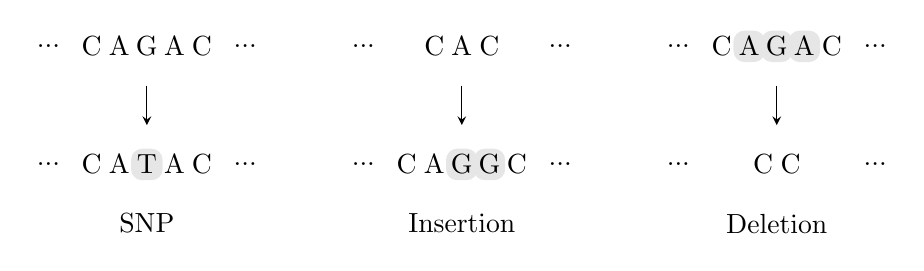
\begin{tikzpicture}
  % SNP
  \node at(.7,0)[rounded corners,minimum width=.4cm,minimum height=.4cm, fill=variantcolor](variant){};
  % lower
  \node at(-.55,0)(){...};
  \node at(0,0)(){C};
  \node at(.35,0)(){A};
  \node at(.7,0)(){T};
  \node at(1.05,0)(){A};
  \node at(1.4,0)(){C};
  \node at(1.95,0)(){...};
  % arrow
  \draw [-stealth](.7,1) -- (.7,.5);
  % upper
  \node at(-.55,1.5)(){...};
  \node at(0,1.5)(){C};
  \node at(.35,1.5)(){A};
  \node at(.7,1.5)(){G};
  \node at(1.05,1.5)(){A};
  \node at(1.4,1.5)(){C};
  \node at(1.95,1.5)(){...};
  \node at(.7,-.75)(){\smaller{SNP}};
  % Insertion
  \node at(.7+4,0)[rounded corners,minimum width=.4cm,minimum height=.4cm, fill=variantcolor](variant){};
  \node at(1.05+4,0)[rounded corners,minimum width=.4cm,minimum height=.4cm, fill=variantcolor](variant){};
  % lower
  \node at(-.55+4,0)(){...};
  \node at(0+4,0)(){C};
  \node at(.35+4,0)(){A};
  \node at(.7+4,0)(){G};
  \node at(1.05+4,0)(){G};
  \node at(1.4+4,0)(){C};
  \node at(1.95+4,0)(){...};
  % arrow
  \draw [-stealth](.7+4,1) -- (.7+4,.5);
  % upper
  \node at(-.55+4,1.5)(){...};
  \node at(.7+4-.35,1.5)(){C};
  \node at(.7+4,1.5)(){A};
  \node at(.7+4+.35,1.5)(){C};
  \node at(1.95+4,1.5)(){...};
  \node at(.7+4,-.75)(){\smaller{Insertion}};
  % Deletion
  \node at(.7+8,1.5)[rounded corners,minimum width=.4cm,minimum height=.4cm, fill=variantcolor](variant){};
  \node at(1.05+8,1.5)[rounded corners,minimum width=.4cm,minimum height=.4cm, fill=variantcolor](variant){};
  \node at(.35+8,1.5)[rounded corners,minimum width=.4cm,minimum height=.4cm, fill=variantcolor](variant){};
  % lower
  \node at(-.55+8,0)(){...};
  \node at(.525+8,0)(){C};
  \node at(.525+.35+8,0)(){C};
  \node at(1.95+8,0)(){...};
  % arrow
  \draw [-stealth](.7+8,1) -- (.7+8,.5);
  % upper
  \node at(-.55+8,1.5)(){...};
  \node at(0+8,1.5)(){C};
  \node at(.35+8,1.5)(){A};
  \node at(.7+8,1.5)(){G};
  \node at(1.05+8,1.5)(){A};
  \node at(1.4+8,1.5)(){C};
  \node at(1.95+8,1.5)(){...};
  \node at(.7+8,-.75)(){\smaller{Deletion}};
\end{tikzpicture}
}
\caption{
  An illustration demonstrating how three types of variants can manifest when aligning sequenced reads to a reference genome.
  From left to right: a single nucleotide polymorphism (SNP), an insertion (indel), and a deletion (indel).
}
\label{background:variant_and_variant_calling:figures:variants}
\end{center}
\end{figure}

The software tool KAGE, which is described in section \ref{background:kage}, focuses on genotyping SNPs and indels.

A common way to represent genome sequence variations is to encode them according to the \textit{Variant Call Format} (VCF) file format.
The VCF file format encodes a single variant per line, and each line contains a number of columns where each column encodes a particular piece of information about the associated variant, such as \cite{vcf}:
\begin{compactenum}
  \item
    CHROM: an identifier for the reference sequence used, \textit{i}.\textit{e}. the sequence against which the sequenced reads varies.
  \item
    POS: the position along the reference sequence where it varies against the sequenced reads.
  \item
    ID: an identifier for the variantion.
  \item
    REF: the reference base (or bases) found at the POS position in the reference sequence.
  \item
    ALT: a list of the alternative base (or bases) found at this POS position.
\end{compactenum}
While more columns are usually present, this encapsulated the necessary knowledge about variants and their representation needed for this thesis.

\definecolor{variantcolor}{RGB}{230,230,230}

\begin{figure}[H]
\begin{center}
\scalebox{1}{
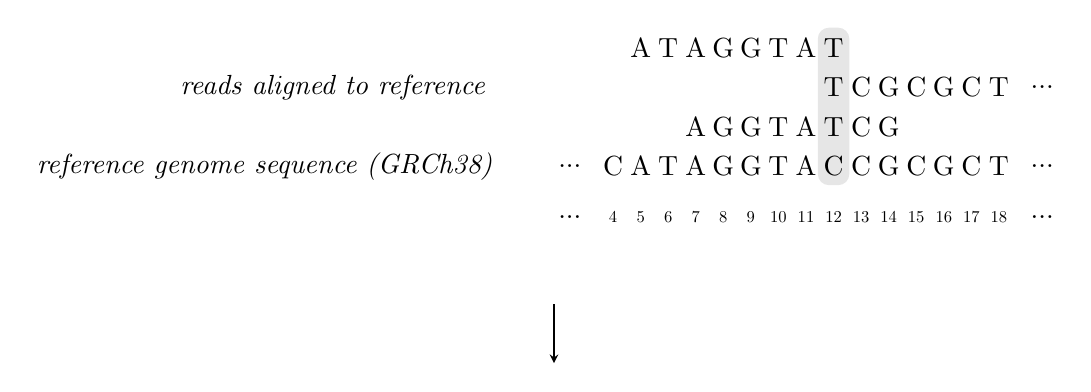
\begin{tikzpicture}
  % texts
  \node at(-4.37,0)(){\smaller\textit{reference genome sequence (GRCh38)}};
  \node at(-3.5,1)(){\smaller\textit{reads aligned to reference}};
  % variant color box
  \node at(2.85,.76)[rounded corners,minimum width=0.4cm,minimum height=2cm, fill=variantcolor](variant){};
  % indices
  \node at(-.5,-.65)(){...};
  \node at(.05,-.65)(){\scalebox{.6}{4}};
  \node at(.40,-.65)(){\scalebox{.6}{5}};
  \node at(.75,-.65)(){\scalebox{.6}{6}};
  \node at(1.1,-.65)(){\scalebox{.6}{7}};
  \node at(1.45,-.65)(){\scalebox{.6}{8}};
  \node at(1.8,-.65)(){\scalebox{.6}{9}};
  \node at(2.15,-.65)(){\scalebox{.6}{10}};
  \node at(2.5,-.65)(){\scalebox{.6}{11}};
  \node at(2.85,-.65)(){\scalebox{.6}{12}};
  \node at(3.2,-.65)(){\scalebox{.6}{13}};
  \node at(3.55,-.65)(){\scalebox{.6}{14}};
  \node at(3.9,-.65)(){\scalebox{.6}{15}};
  \node at(4.25,-.65)(){\scalebox{.6}{16}};
  \node at(4.6,-.65)(){\scalebox{.6}{17}};
  \node at(4.95,-.65)(){\scalebox{.6}{18}};
  \node at(5.5,-.65)(){...};
  % lower nodes
  \node at(-.5,0)(){...};
  \node at(.05,0)(){C};
  \node at(.40,0)(){A};
  \node at(.75,0)(){T};
  \node at(1.1,0)(){A};
  \node at(1.45,0)(){G};
  \node at(1.8,0)(){G};
  \node at(2.15,0)(){T};
  \node at(2.5,0)(){A};
  \node at(2.85,0)(){C};
  \node at(3.2,0)(){C};
  \node at(3.55,0)(){G};
  \node at(3.9,0)(){C};
  \node at(4.25,0)(){G};
  \node at(4.6,0)(){C};
  \node at(4.95,0)(){T};
  \node at(5.5,0)(){...};
  % read 1
  \node at(1.1,.5)(){A};
  \node at(1.45,.5)(){G};
  \node at(1.8,.5)(){G};
  \node at(2.15,.5)(){T};
  \node at(2.5,.5)(){A};
  \node at(2.85,.5)(){T};
  \node at(3.2,.5)(){C};
  \node at(3.55,.5)(){G};
  % read 2
  \node at(2.85,1)(){T};
  \node at(3.2,1)(){C};
  \node at(3.55,1)(){G};
  \node at(3.9,1)(){C};
  \node at(4.25,1)(){G};
  \node at(4.6,1)(){C};
  \node at(4.95,1)(){T};
  \node at(5.5,1)(){...};
  % read 3
  \node at(.40,1.5)(){A};
  \node at(.75,1.5)(){T};
  \node at(1.1,1.5)(){A};
  \node at(1.45,1.5)(){G};
  \node at(1.8,1.5)(){G};
  \node at(2.15,1.5)(){T};
  \node at(2.5,1.5)(){A};
  \node at(2.85,1.5)(){T};
  % down arrow
  \draw [-stealth](-.7,-1.75) -- (-.7,-2.5);
\end{tikzpicture}
}

\vspace{1em}
\small{example.vcf}
\begin{lstlisting}[style=vcf]
##fileformat=VCFv4.2
##reference=GRCh38
#CHROM POS     ID  REF  ALT  QUAL FILTER INFO
1      12      .   C    T    30   PASS   NS=3;DP=3
...
\end{lstlisting}
\caption{
An illustration of how sequenced reads can be aligned against a reference genome sequence in order to call variants present in the genome of the sequenced individual. The called variant in the illustration is then stored in a variant call format (VCF) file where the chromosome identifier, 1-indexed position along the chromosome reference sequence, an identifier for the variant, the allele or alleles present in the reference sequence, the alternative variant allele or alleles, along with a number of other parameters are used to represent each variant.
}
\label{background:variant_and_variant_calling:figures:variant_calling}
\end{center}
\end{figure}
